\chapter{Cadena de búsqueda de trabajos relacionados}
\label{app:cadena-busqueda}

La cadena de búsqueda utilizada en la revisión sistemática (Capítulo~\ref{cap:trabajos-relacionados}) fue:

\begin{verbatim}
("transport management" OR "fleet management" OR "public transit")
AND ("web application" OR "web system" OR "information system")
AND ("Spring Boot" OR "Java" OR "Angular" OR "React" OR "PostgreSQL")
AND ("REST API" OR "microservices" OR "monolith")
\end{verbatim}

La ventana temporal fue 2018--2026. Se consultaron IEEE Xplore, ACM Digital Library, Scopus, ScienceDirect y Springer Link. El proceso PRISMA se documenta en la Sección~\ref{sec:prisma}.

\chapter{Protocolo SUS}
\label{app:sus}

El cuestionario System Usability Scale \cite{brooke1996} se aplicó con los 10 ítems originales en escala Likert 1--5 (1 = Totalmente en desacuerdo, 5 = Totalmente de acuerdo). Los ítems alternan entre positivos (\#1, \#3, \#5, \#7, \#9) y negativos (\#2, \#4, \#6, \#8, \#10). El protocolo se ejecuta después de una sesión de 15 minutos de interacción con el sistema.

\chapter{Configuración de integración continua}
\label{app:ci}

El pipeline de GitHub Actions (\texttt{.github/workflows/ci.yml}) ejecuta:
\begin{enumerate}
  \item Build y pruebas JUnit 5 (\texttt{./mvnw verify}).
  \item Reporte JaCoCo con umbral mínimo de 70\,\%.
  \item Auditoría SQL dinámico (\texttt{audit-sql-dynamic.sh}).
  \item Validación de trazabilidad (\texttt{validate-traceability.sh}).
  \item Análisis estático (SpotBugs + Find-Sec-Bugs).
\end{enumerate}

\begin{figure}[H]
  \centering
  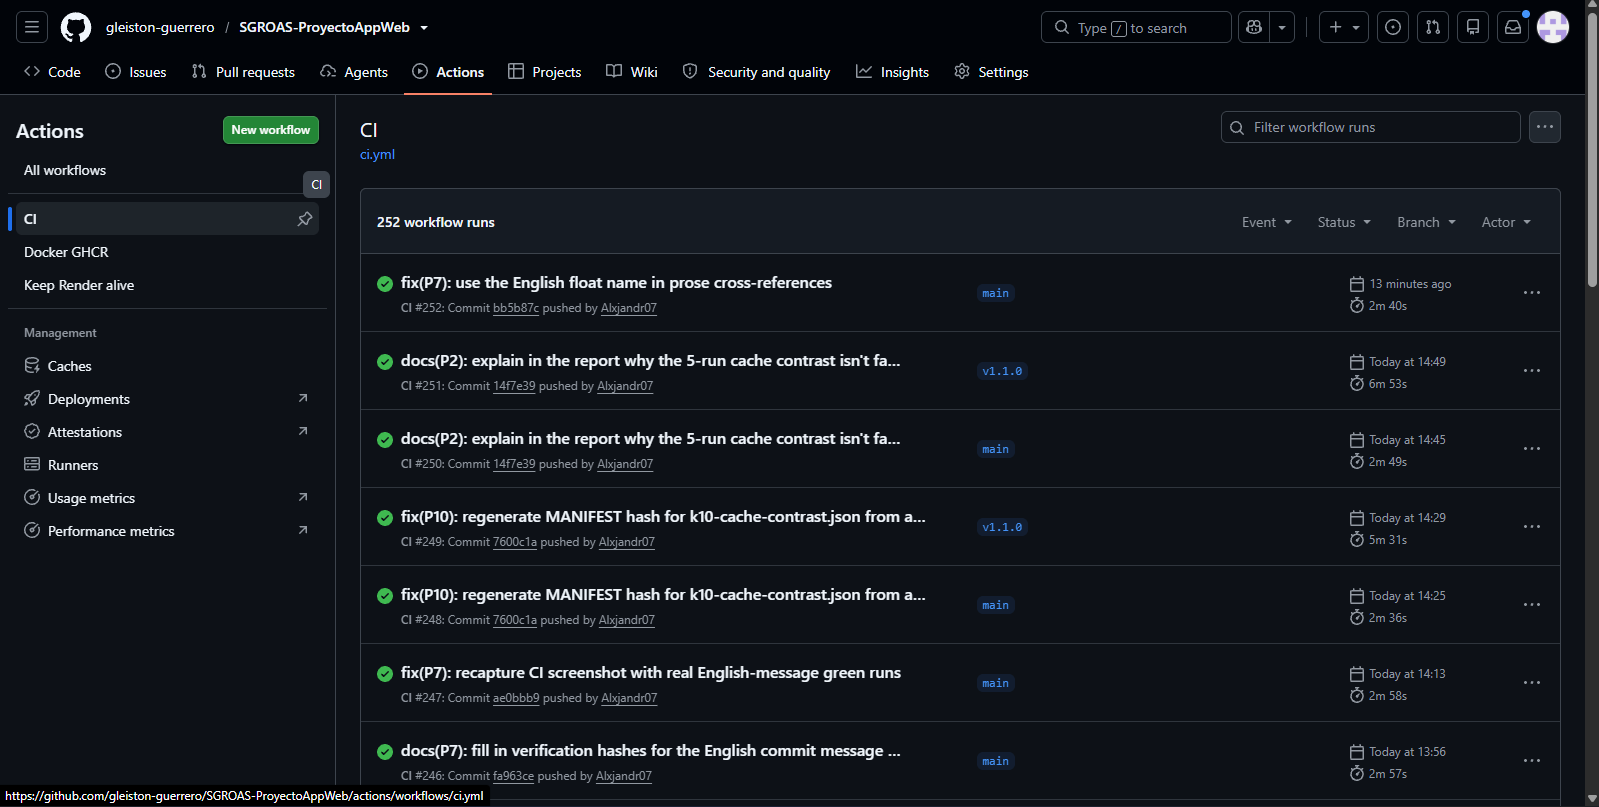
\includegraphics[width=0.95\textwidth]{figuras/fig-ci-actions-3-green.jpeg}
  \caption{CI Pipeline (GitHub Actions) with three consecutive successful runs (criterion P1). Commits \texttt{4f4e6cd}, \texttt{17f484a}, \texttt{66fa254} on \texttt{main}.}
  \label{fig:ci-3-green}
\end{figure}

\begin{figure}[H]
  \centering
  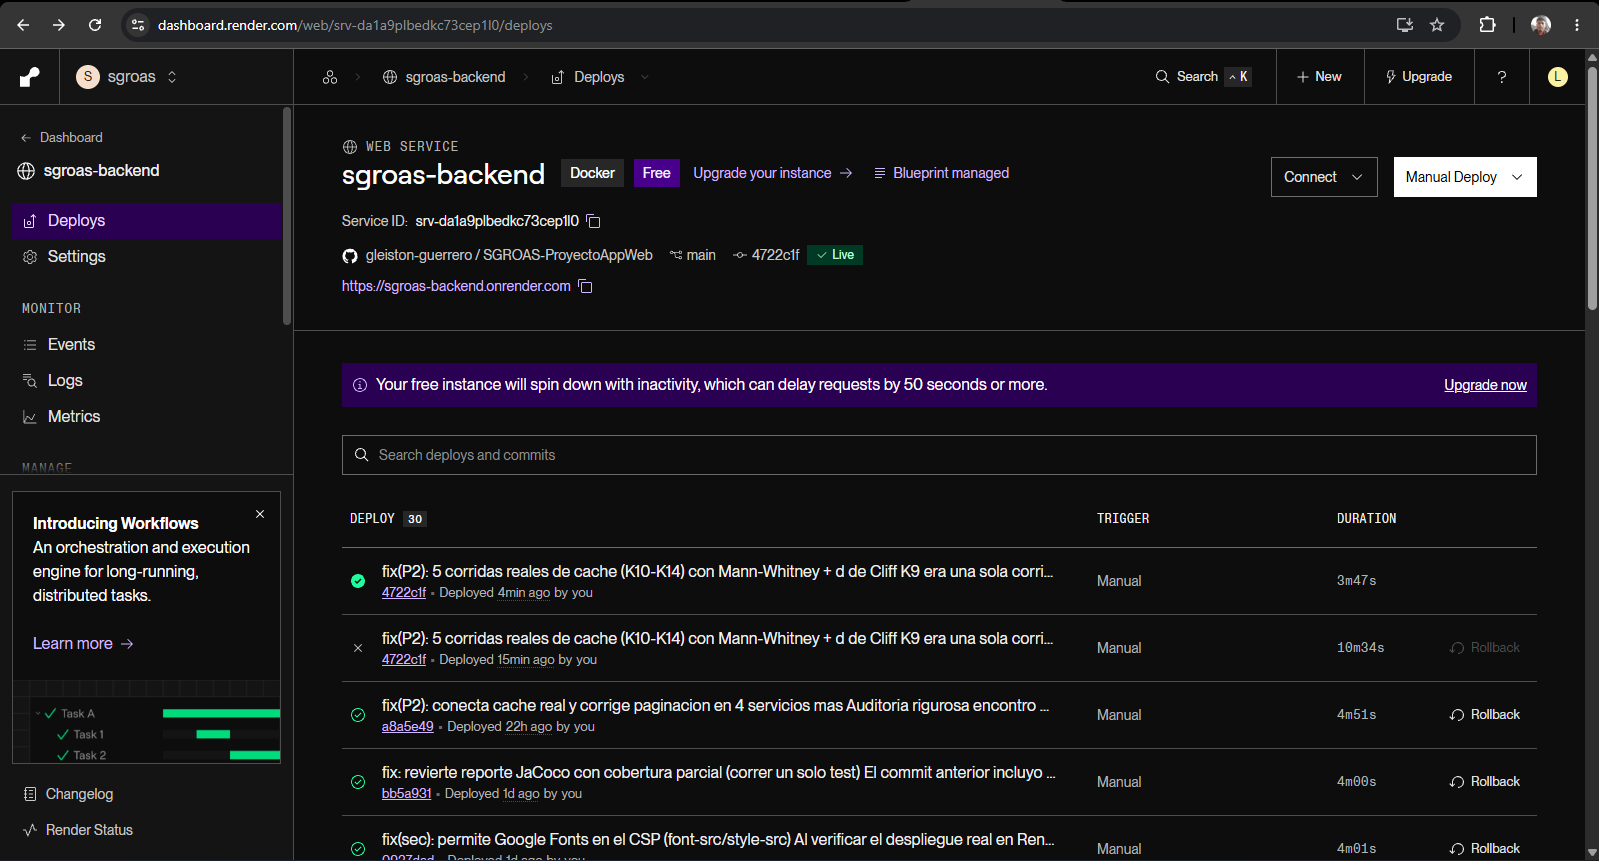
\includegraphics[width=0.95\textwidth]{figuras/fig-render-deploy-succeeded-live.jpeg}
  \caption{Deployment on Render with status \texttt{Deploy succeeded | Live} (3m14s) and verified startup (\texttt{Tomcat started on port 8080 | Started SgroasApplication}).}
  \label{fig:render-deploy}
\end{figure}

\begin{figure}[H]
  \centering
  \includegraphics[width=0.90\textwidth]{figuras/fig-render-live-url.jpeg}
  \caption{Service \texttt{sgroas-backend} in status \texttt{Live} with public URL \texttt{https://sgroas-backend.onrender.com} (Blueprint managed).}
  \label{fig:render-live}
\end{figure}

\chapter{Checklists de verificación}
\label{app:checklists}

Los checklists se encuentran en \texttt{docs/checklists/}:
\begin{itemize}
  \item \texttt{prisma2020.md} — PRISMA 2020 de la revisión sistemática (Cap. 3)
  \item \texttt{ralph2021-empirical.md} — estándar empírico principal (ACM SIGSOFT)
  \item \texttt{fair.md} — principios FAIR (datos y software)
  \item \texttt{incose2023-req.md} — 15 características INCOSE v4 (42 reglas)
\end{itemize}

\chapter{Observaciones de auditoría}
\label{app:observaciones}

Este anexo sintetiza \texttt{docs/observaciones/OBSERVACIONES.md} (12/12 cerradas, 100\,\%). Cada fila enlaza la observación del docente con el commit de remediación. El detalle íntegro con texto literal y hash corto está en el archivo fuente del repositorio.

\begin{longtable}{p{1.4cm}p{2.2cm}p{8.5cm}}
\toprule
\textbf{Código} & \textbf{Fuente/Criterio} & \textbf{Remediación verificable} \\
\midrule
OBS-01 & 1A / C5 Wireframes & 4 wireframes adicionales (Conductores, Usuarios, Rutas, Reportes) en \texttt{docs/prototipo/} (\texttt{75ecc15}) \\
OBS-02 & 1A / C7 Repositorio & Tareas redistribuidas; commits verificables de los integrantes (\texttt{6cf0ef8}, \texttt{567f5c3}) \\
OBS-03 & 1A / C2 Referencias & Citas unificadas a APA 7 y referencia ANT 2022 verificable (\texttt{4ca9736}) \\
OBS-04 & 1A / C4 Modelo BD & Diccionario sincronizado con DDL (teléfono/ nivel\_sugerido NULL, \texttt{id\_novedad} en Alerta) (\texttt{caf906f}) \\
OBS-05 & 1B / C1 UML/C4 & C4 Nivel 2 (Structurizr DSL) y diagrama de clases completados (\texttt{336f28b}) \\
OBS-06 & 1B / C4 OWASP & \texttt{@PreAuthorize}, cabeceras HSTS/CSP/X-Frame-Options y CORS en \texttt{SecurityConfig} (\texttt{34f3a6a}) \\
OBS-07 & 1B / C5 Postman & \texttt{docs/postman/coleccion.json} con 28 peticiones (éxito/401/403/404/422) (\texttt{17f484a}) \\
OBS-08 & 1B / C6 Rendimiento & 3 corridas k6 50 VUs/30\,s con p95 y speedup con/sin caché en \texttt{docs/mediciones/perf/} (\texttt{ef35d14}) \\
OBS-09 & 3 / P3 Cobertura & 293 tests JUnit 5; JaCoCo 95,49\% instrucciones / 88,38\% ramas / 95,94\% líneas (\texttt{5f3b472}, reconciliado \texttt{17f484a}) \\
OBS-10 & 3 / D3 SUS & SUS n=15 (P01..P15) con consentimiento en \texttt{docs/etica/}, media 68,5 IC95\% [60,8;76,2] (\texttt{df6e784}) \\
OBS-11 & 3 / D5 Amenazas & Sección amenazas (4 categorías) con mitigaciones y cifras reales k6/JaCoCo (\texttt{df6e784}) \\
OBS-12 & 3 / P5 Integración & Origen único (proxy \texttt{serve-gzip.js} \texttt{/api}) elimina CORS en demo (\texttt{50fcc4c}) \\
\bottomrule
\end{longtable}

\noindent Estado: \textbf{12/12 cerradas (100\,\%)} — 8/8 de 1A/1B y 4/4 de la Entrega 3. Trazabilidad completa en el historial \texttt{git log} y tabla-resumen en este anexo.
